\chapter{Supplementary material on timeseries data}

\section{Further examples of trajectory data}

Find below the trajectory timeseries visualisation plots - as figure 3.2 - for the locations in figure 3.1. Each figure contains plots (a-d) of TX1day T’ decompositions for years 1980 to 2020. The x-axis is logarithmic to better represent the recent history. The trajectory yielding the largest final $T'$ among all years is colored red, the time-mean of all trajectories in black and the inter-quantile range is highlighted in light blue. Plot (e) shows the (auto-)correlation between the final $T'$ and the $T'$ at different lags for the event and each contributor. Plot (f) shows the (cross-)correlation between the final event $T'$ and the $T'$ at different lags for each contributor. They are computed for all samples that have genesis time earlier than the considered time-lag.

\begin{figure}[h]
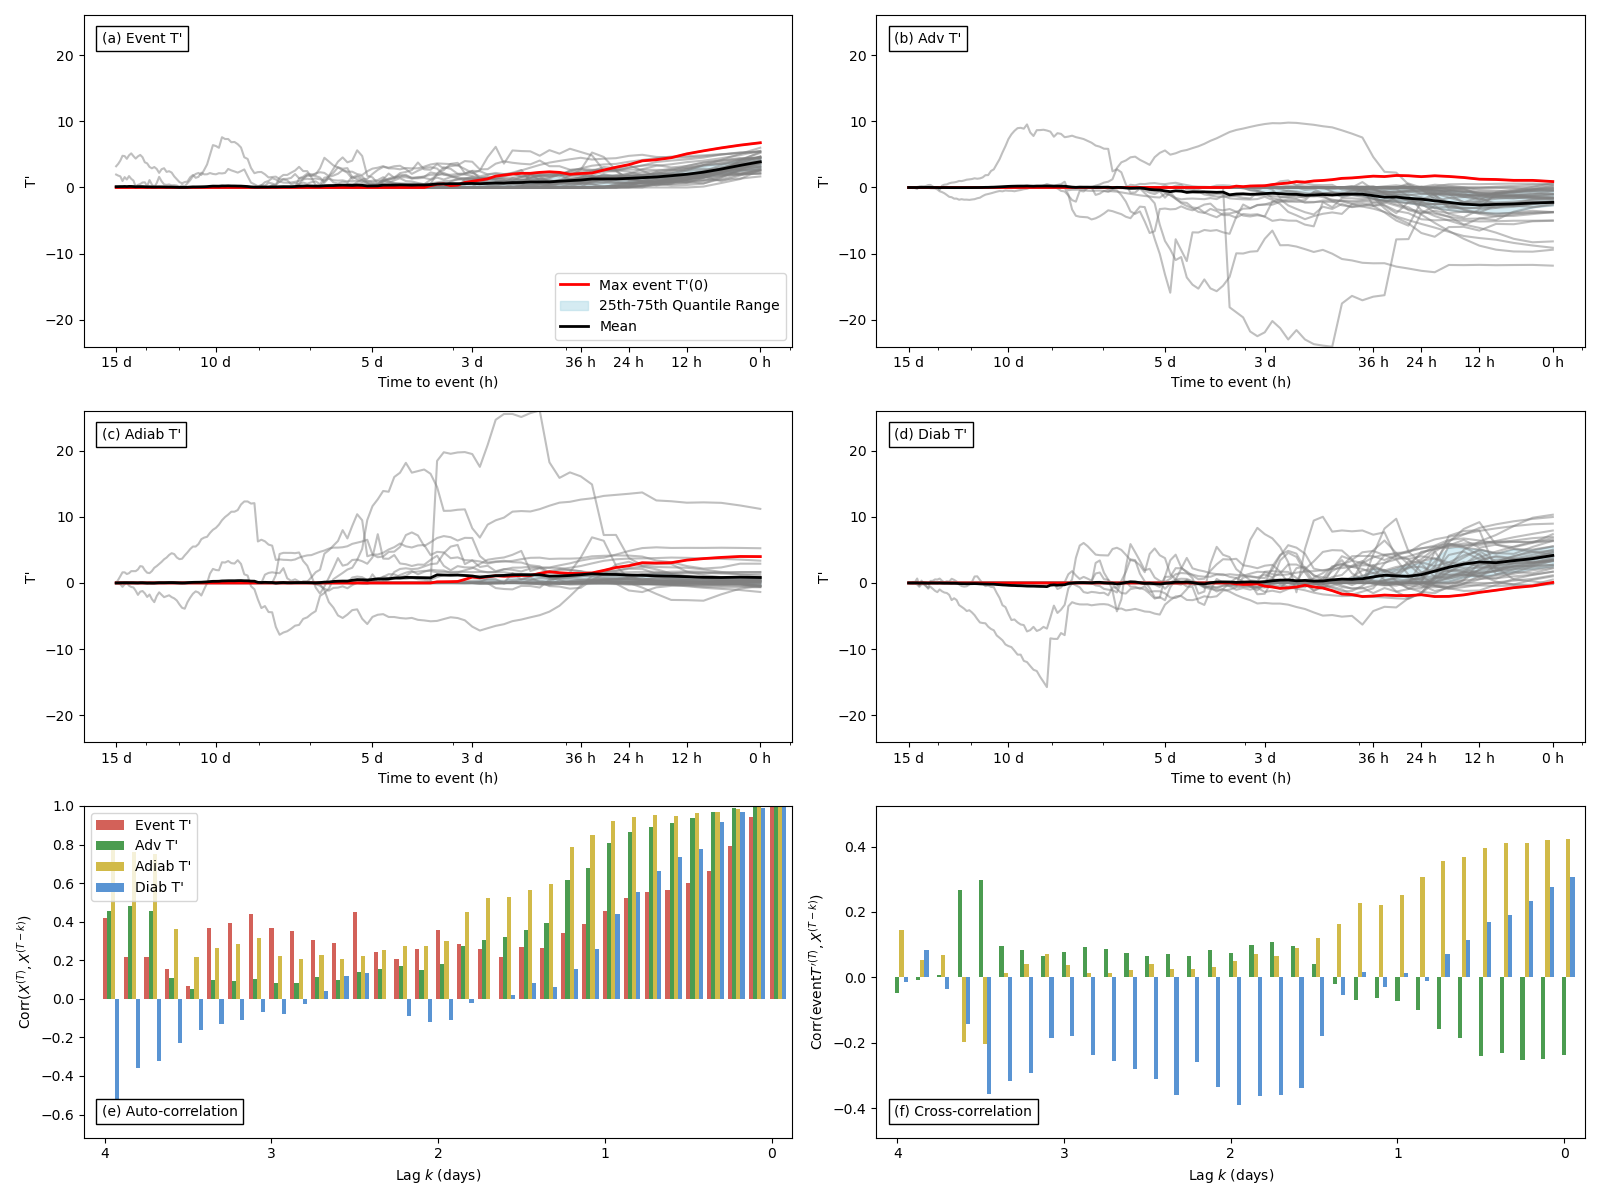
\includegraphics[width=\textwidth]{images/sup1.png}
\caption{Gridpoint 28.5N 77E located in the vicinity of New Delhi (India)}
\end{figure}

\begin{figure}[h]
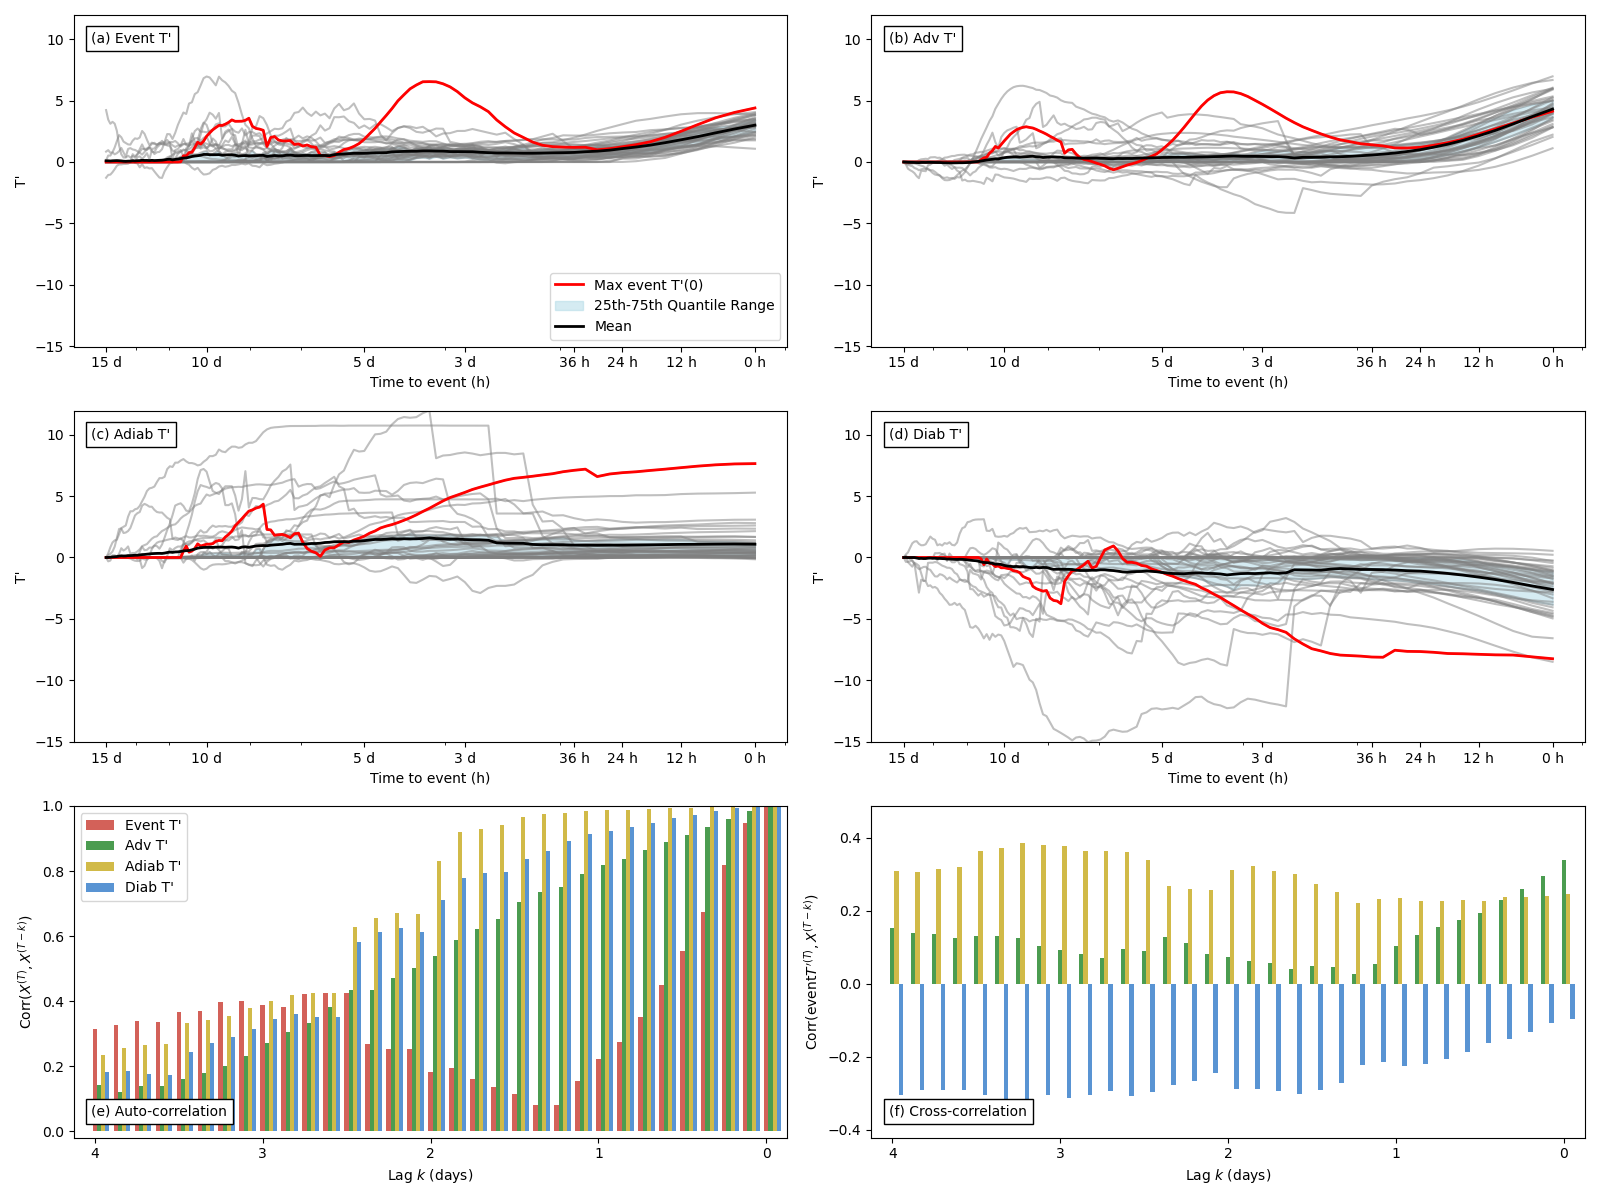
\includegraphics[width=\textwidth]{images/sup2.png}
\caption{Gridpoint 45N 30W located in the middle of the Atlantic ocean.}
\end{figure}

\begin{figure}[h]
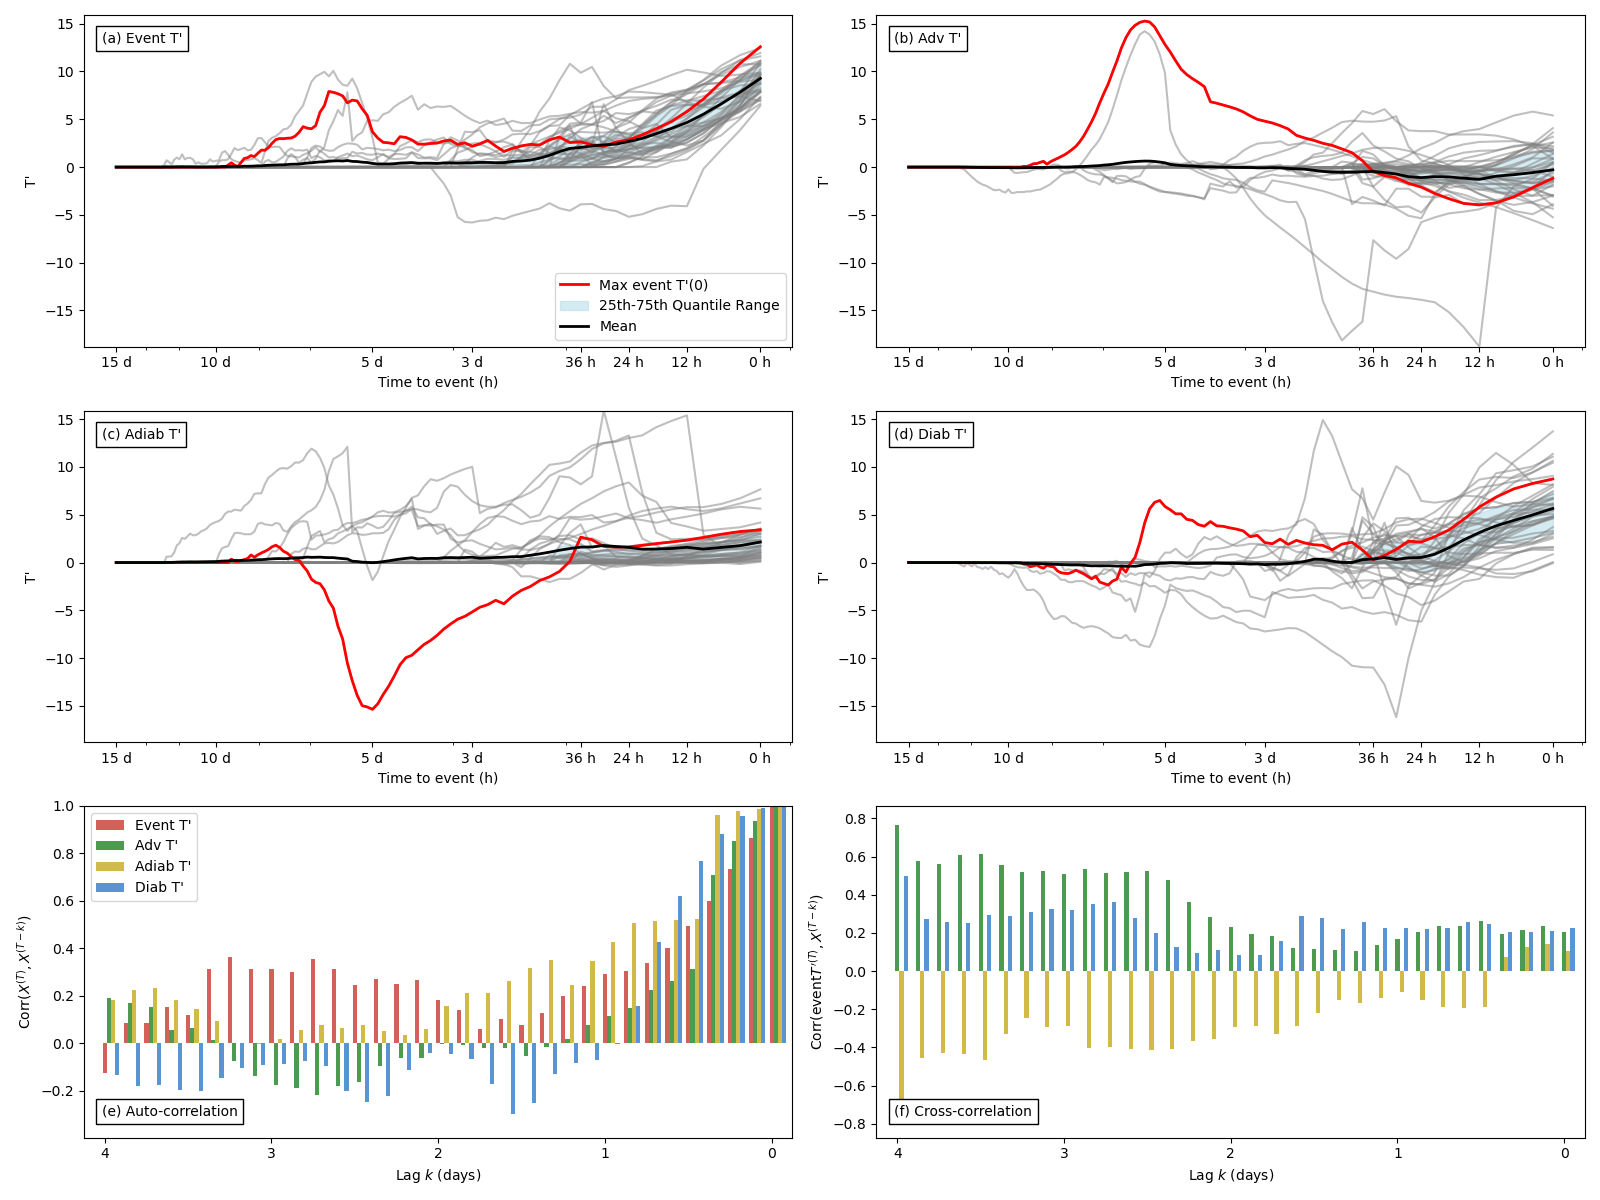
\includegraphics[width=\textwidth]{images/sup3.png}
\caption{Gridpoint 32S 116E located in the vicinity of Perth (Australia).}
\end{figure}

%%% Local Variables: 
%%% mode: latex
%%% TeX-master: "MasterThesisSfS"
%%% End: 
